\documentclass{beamer}

% Choose a presentation theme
\usetheme{Madrid}
\usecolortheme{default}

% Required packages for math symbols and drawing Hasse diagrams
\usepackage{amsmath}
\usepackage{amssymb}
\usepackage{tikz}

\title{Mathematics for Computing}
\subtitle{Assignment 1}
\author{Alen Francis Joseph}

% Here is the "sub thing" - you can change this to your actual college/ID
\institute{Semester 1 - M.Tech in Computer Science and Engineering with specialization in Data Science and Artificial Intelligence \\ \vspace{0.2cm} \small Department of Computer Science, CUSAT} 
\date{\today}

\begin{document}

% Title Slide
\begin{frame}
    \titlepage
\end{frame}

% Slide 1: Definition
\begin{frame}{Definition of a Set}
    \begin{block}{What is a Set?}
        A set is a well-defined unordered collection of distinct elements.
    \end{block}
    
    \vspace{0.5cm}
    
    \textbf{Example: Positive odd integers less than 10}
    \begin{gather*}
        S = \{1, 3, 5, 7, 9\} \\
        S = \{ x \mid x \in \mathbb{Z}^+ \land (x < 10) \land (\exists k \in \mathbb{Z} : x = 2k + 1) \}
    \end{gather*}
\end{frame}

% Slide 2
\begin{frame}{Some more examples}
    \textbf{1. Perfect Squares}
    \begin{gather*}
        A = \{1, 4, 9, 16, 25, 36, 49\} \\
        A = \{ x \mid x \in \mathbb{Z}^+ \land (\exists n \in \mathbb{Z} : (1 \le n \le 7) \land (x = n^2)) \}
    \end{gather*}
    
    \vspace{0.5cm}
    
    \textbf{2. Powers of 2}
    \begin{gather*}
        B = \{1, 2, 4, 8, 16, 32, 64\} \\
        B = \{ x \mid x \in \mathbb{Z}^+ \land (\exists n \in \mathbb{Z} : (0 \le n \le 6) \land (x = 2^n)) \}
    \end{gather*}
\end{frame}

% Slide 3
\begin{frame}{Some more examples}
    \textbf{3. Prime Numbers in a Range}
    \begin{gather*}
        C = \{2, 3, 5, 7, 11, 13, 17, 19\} \\
        C = \{ x \mid x \in \mathbb{Z}^+ \land (1 < x < 20) \land \\
        (\forall a, b \in \mathbb{Z}^+ : (x = ab) \implies (a = 1 \lor b = 1)) \}
    \end{gather*}
    
    \vspace{0.5cm}
    
    \textbf{4. Absolute Value Inequality}
    \begin{gather*}
        D = \{-1, 0, 1, 2, 3, 4\} \\
        D = \{ x \mid x \in \mathbb{Z} \land |2x - 3| \le 5 \}
    \end{gather*}
\end{frame}

% Slide 4
\begin{frame}{Some more examples}
    \textbf{5. Modulo Arithmetic}
    \begin{gather*}
        E = \{3, 8, 13, 18, 23\} \\
        E = \{ x \mid x \in \mathbb{Z}^+ \land (x < 25) \land (\exists k \in \mathbb{Z} : x = 5k + 3) \}
    \end{gather*}
    
    \vspace{0.5cm}
    
    \textbf{6. Divisors of a Number}
    \begin{gather*}
        F = \{1, 2, 3, 4, 6, 8, 12, 24\} \\
        F = \{ x \mid x \in \mathbb{Z}^+ \land (\exists k \in \mathbb{Z}^+ : 24 = xk) \}
    \end{gather*}
\end{frame}

% Slide 5
\begin{frame}{Some more examples}
    \textbf{7. Roots of a Polynomial}
    \begin{gather*}
        G = \{-2, 0, 2\} \\
        G = \{ x \mid x \in \mathbb{Z} \land x^3 - 4x = 0 \}
    \end{gather*}
    
    \vspace{0.5cm}
    
    \textbf{8. Factorials}
    \begin{gather*}
        H = \{1, 2, 6, 24, 120\} \\
        H = \{ x \mid x \in \mathbb{Z}^+ \land (\exists n \in \mathbb{Z}^+ : (n \le 5) \land (x = n!)) \}
    \end{gather*}
\end{frame}

% Slide 6
\begin{frame}{Some more examples}
    \textbf{9. Boolean Cartesian Product}
    \begin{gather*}
        I = \{(0,0), (0,1), (1,0), (1,1)\} \\
        I = \{ (x, y) \mid x \in \mathbb{Z} \land y \in \mathbb{Z} \land (0 \le x \le 1) \land (0 \le y \le 1) \}
    \end{gather*}
    
    \vspace{0.5cm}
    
    \textbf{10. Intersecting Conditions}
    \begin{gather*}
        J = \{10, 12, 14, 16, 18\} \\
        J = \{ x \mid x \in \mathbb{Z}^+ \land (10 \le x < 20) \land (\exists k \in \mathbb{Z} : x = 2k) \}
    \end{gather*}
\end{frame}

% Slide 7: Types of Sets (Finite, Infinite, Countable)
\begin{frame}{Types of Sets (AI \& DS Context)}
    \textbf{1. Finite Set} \\
    \hspace*{1.5em}A set with a strictly limited number of elements. \\
    \begin{tabular}{@{\hspace{1.5em}}l@{\hspace{0.5em}}p{0.75\textwidth}@{}}
        \textit{E.g:} & The discrete set of activation functions evaluated during hyperparameter tuning:
    \end{tabular}
    \[ A_{func} = \{\text{ReLU}, \text{Sigmoid}, \text{Tanh}\} \]
    
    \textbf{2. Infinite Set} \\
    \hspace*{1.5em}A set with an unlimited number of elements. \\
    \begin{tabular}{@{\hspace{1.5em}}l@{\hspace{0.5em}}p{0.75\textwidth}@{}}
        \textit{E.g:} & The continuous state space or weight space in a neural network: 
    \end{tabular}
    \[ W = \mathbb{R}^n \]
    
    \textbf{3. Countable Set} \\
    \hspace*{1.5em}A set whose elements can be mapped 1-to-1 with natural numbers. \\
    \begin{tabular}{@{\hspace{1.5em}}l@{\hspace{0.5em}}p{0.75\textwidth}@{}}
        \textit{E.g:} & The sequential set of training epochs in a model:
    \end{tabular}
    \[ E = \{1, 2, 3, \dots\} \]
\end{frame}

% Slide 8: Types of Sets (Null, Singleton, Cardinality)
\begin{frame}{Types of Sets (AI \& DS Context)}
    \textbf{4. Null (Empty) Set ($\emptyset$)} \\
    \hspace*{1.5em}A set containing no elements. \\
    \begin{tabular}{@{\hspace{1.5em}}l@{\hspace{0.5em}}p{0.75\textwidth}@{}}
        \textit{E.g:} & The set of false positive predictions in a flawless, 100\% precision classification model: 
    \end{tabular}
    \[ FP = \emptyset \]
    
    \vspace{0.3cm}
    
    \textbf{5. Singleton Set} \\
    \hspace*{1.5em}A set containing exactly one element. \\
    \begin{tabular}{@{\hspace{1.5em}}l@{\hspace{0.5em}}p{0.75\textwidth}@{}}
        \textit{E.g:} & The optimal weight vector $\theta^*$ that represents the single global minimum of a strictly convex loss function:
    \end{tabular}
    \[ M = \{\theta^*\} \]
    
    \textbf{6. Cardinality ($|S|$)} \\
    \hspace*{1.5em}The total number of unique elements in a set. \\
    \begin{tabular}{@{\hspace{1.5em}}l@{\hspace{0.5em}}p{0.75\textwidth}@{}}
        \textit{E.g:} & The dimensionality of a dataset. If a dataset has $n$ unique features, the cardinality of the feature set $F$ is:
    \end{tabular}
    \[ |F| = n \]
\end{frame}

% Slide 9: Types of Sets (Equal vs Equivalent)
\begin{frame}{Types of Sets (AI \& DS Context)}
    \textbf{7. Equal Sets ($A = B$)} \\
    \hspace*{1.5em}Sets containing the exact same elements, regardless of order. \\
    \begin{tabular}{@{\hspace{1.5em}}l@{\hspace{0.5em}}p{0.75\textwidth}@{}}
        \textit{E.g:} & Defining unique class labels for a computer vision model in different orders yields equal sets.
    \end{tabular}
    \begin{gather*}
        C_1 = \{\text{Cat}, \text{Dog}\} \\
        C_2 = \{\text{Dog}, \text{Cat}\} \\
        \implies C_1 = C_2
    \end{gather*}
    
    \textbf{8. Equivalent Sets ($|A| = |B|$)} \\
    \hspace*{1.5em}Sets possessing the exact same cardinality (number of elements). \\
    \begin{tabular}{@{\hspace{1.5em}}l@{\hspace{0.5em}}p{0.75\textwidth}@{}}
        \textit{E.g:} & An autoencoder where the set of input layer neurons ($I$) maps one-to-one with the set of output layer neurons ($O$).
    \end{tabular}
    \[ |I| = |O| \]
\end{frame}

% Slide 10: Types of Sets (Subset, Superset, Universal)
\begin{frame}{Types of Sets (AI \& DS Context)}
    \textbf{9. Subset ($A \subseteq B$)} \\
    \hspace*{1.5em}A set where all its elements are contained within another set $B$. \\
    \begin{tabular}{@{\hspace{1.5em}}l@{\hspace{0.5em}}p{0.75\textwidth}@{}}
        \textit{E.g:} & In Support Vector Machines (SVM), the set of support vectors ($SV$) is a subset of the training data ($D$).
    \end{tabular}
    \[ SV \subseteq D \]
    
    \textbf{10. Superset ($B \supseteq A$)} \\
    \hspace*{1.5em}A set that contains all the elements of another set $A$. \\
    \begin{tabular}{@{\hspace{1.5em}}l@{\hspace{0.5em}}p{0.75\textwidth}@{}}
        \textit{E.g:} & A massive pre-training text corpus ($C$) acts as a superset containing all the text in a smaller fine-tuning dataset ($F$).
    \end{tabular}
    \[ C \supseteq F \]
    
    \textbf{11. Universal Set ($U$)} \\
    \hspace*{1.5em}The overarching set containing all objects under consideration. \\
    \begin{tabular}{@{\hspace{1.5em}}l@{\hspace{0.5em}}p{0.75\textwidth}@{}}
        \textit{E.g:} & In NLP, the Universal Set is the entire language vocabulary corpus from which words are drawn.
    \end{tabular}
\end{frame}

% Slide 11: Types of Sets (Power Set)
\begin{frame}{Types of Sets (AI \& DS Context)}
    \textbf{12. Power Set ($\mathcal{P}(S)$)} \\
    \hspace*{1.5em}The set of all possible subsets of $S$, including the null set and $S$ itself. \\
    \begin{tabular}{@{\hspace{1.5em}}l@{\hspace{0.5em}}p{0.75\textwidth}@{}}
        \textit{E.g:} & In exhaustive feature selection, if we have a small feature set $F = \{f_1, f_2\}$, the power set represents every possible combination of features a model could be trained on:
    \end{tabular}
    \[ \mathcal{P}(F) = \{\emptyset, \{f_1\}, \{f_2\}, \{f_1, f_2\}\} \]
    
    \begin{tabular}{@{\hspace{1.5em}}l@{\hspace{0.5em}}p{0.75\textwidth}@{}}
        \textit{Note:} & If the dataset has $n$ unique features ($|F| = n$), the cardinality of the power set is:
    \end{tabular}
    \[ |\mathcal{P}(F)| = 2^n \]
    \begin{tabular}{@{\hspace{1.5em}}l@{\hspace{0.5em}}p{0.75\textwidth}@{}}
        & This explains why exhaustive feature search is computationally expensive for large datasets!
    \end{tabular}
\end{frame}

% Slide 12: Inclusion-Exclusion Principle (Definition & Equation)
\begin{frame}{Inclusion-Exclusion Principle}
    \textbf{Definition} \\
    \hspace*{1.5em}A counting technique used to determine the cardinality of the union of overlapping sets by adding the sizes of individual sets and subtracting the sizes of their intersections to correct for overcounting. \\
    
    \vspace{0.4cm}
    
    \textbf{Equation (For 2 and 3 Sets)} \\
    \hspace*{1.5em}For two sets $A$ and $B$:
    \[ |A \cup B| = |A| + |B| - |A \cap B| \]
    
    \hspace*{1.5em}For three sets $A, B$, and $C$:
    \begin{gather*}
        |A \cup B \cup C| = |A| + |B| + |C| - |A \cap B| - |A \cap C| - |B \cap C| \\
        + |A \cap B \cap C|
    \end{gather*}
\end{frame}

% Slide 13: Inclusion-Exclusion Principle (General Form)
\begin{frame}{Inclusion-Exclusion Principle}
    \textbf{General Form} \\
    \hspace*{1.5em}For $n$ finite sets $A_1, A_2, \dots, A_n$, the exact cardinality of their union is formulated as:
    \begin{gather*}
        \left| \bigcup_{i=1}^n A_i \right| = \sum_{i=1}^n |A_i| - \sum_{1 \le i < j \le n} |A_i \cap A_j| \\
        + \sum_{1 \le i < j < k \le n} |A_i \cap A_j \cap A_k| - \dots + (-1)^{n-1} \left| \bigcap_{i=1}^n A_i \right|
    \end{gather*}
    
    \vspace{0.4cm}
    
    \begin{tabular}{@{\hspace{1.5em}}l@{\hspace{0.5em}}p{0.75\textwidth}@{}}
        \textit{E.g:} & In Machine Learning probability calculations, this principle is crucial when computing the joint likelihood of multiple overlapping features, ensuring that the intersection of intersecting user behaviors or text features isn't counted multiple times.
    \end{tabular}
\end{frame}

% Slide: Set Operations
\begin{frame}{Set Operations}
\begin{block}{Definition}
Set operations are used to construct new sets from existing ones. The most common operations are Union ($\cup$), Intersection ($\cap$), Difference ($-$), and Complement ($A^c$ or $A'$).
\end{block}
\vspace{0.5cm}
\textbf{Example: Let $A = \{1, 2, 3, 4\}$ and $B = \{3, 4, 5, 6\}$}
\begin{gather*}
\text{Union: } A \cup B = \{1, 2, 3, 4, 5, 6\} \\
\text{Intersection: } A \cap B = \{3, 4\} \\
\text{Difference: } A - B = \{1, 2\}
\end{gather*}
\end{frame}

% Slide: Relations
\begin{frame}{Relations}
\begin{block}{Definition}
A binary relation $R$ from a set $A$ to a set $B$ is a subset of the Cartesian product $A \times B$. If $(a, b) \in R$, we say $a$ is related to $b$, often denoted as $aRb$.
\end{block}
\vspace{0.5cm}
\textbf{Example:} Let $A = \{1, 2, 3\}$ and $B = \{x, y\}$. \\
The Cartesian product is:
\begin{gather*}
A \times B = \{(1, x), (1, y), (2, x), (2, y), (3, x), (3, y)\}
\end{gather*}
A relation $R \subseteq A \times B$ could simply be defined as:
\begin{gather*}
R = \{(1, x), (2, y), (3, x)\}
\end{gather*}
\end{frame}

% Slide: Equivalence Relations
\begin{frame}{Equivalence Relations}
\begin{block}{Definition}
A relation $R$ on a set $A$ is an \textbf{equivalence relation} if it satisfies three properties: it is reflexive, symmetric, and transitive. It partitions the set into disjoint subsets called equivalence classes.
\end{block}
\vspace{0.3cm}
\textbf{Example: Congruence Modulo 3} \\
Let $R$ be a relation on integers $\mathbb{Z}$ where $aRb \iff a \equiv b \pmod{3}$.
\begin{itemize}
    \item \textbf{Reflexive:} $a - a = 0$, which is divisible by 3.
    \item \textbf{Symmetric:} If $3 \mid (a - b)$, then $3 \mid (b - a)$.
    \item \textbf{Transitive:} If $3 \mid (a - b)$ and $3 \mid (b - c)$, then $3 \mid (a - c)$.
\end{itemize}
\small \textit{Equivalence classes formed: $[0] = \{\dots, -3, 0, 3, \dots\}$, $[1]$, and $[2]$.}
\end{frame}

% Slide: Chains and Antichains
\begin{frame}{Chains and Anti-chains}
\begin{block}{Chain}
A subset of a partially ordered set (poset) is called a \textbf{chain} if every pair of elements in the subset is comparable (forming a total order).
\end{block}
\begin{block}{Anti-chain}
A subset of a poset is called an \textbf{anti-chain} if no two distinct elements in the subset are comparable to each other.
\end{block}
\vspace{0.2cm}
\textbf{Example: Power set of $S = \{a, b, c\}$ under subset inclusion ($\subseteq$)}
\begin{itemize}
    \item \textbf{Chain:} $\{\emptyset, \{a\}, \{a, b\}, \{a, b, c\}\}$ \\ \small \textit{(Each element is a subset of the next)}
    \item \textbf{Anti-chain:} $\{\{a\}, \{b\}, \{c\}\}$ \\ \small \textit{(None of these are subsets of one another)}
\end{itemize}
\end{frame}

% Slide 14: Partially Ordered Sets (Posets)
\begin{frame}{Partially Ordered Sets (Posets)}
    \textbf{Definition} \\
    \hspace*{1.5em}A partially ordered set (or poset) consists of a set $S$ and a binary relation $\preceq$ that satisfies three properties: it is reflexive, antisymmetric, and transitive.
    \[ (S, \preceq) \]
    
    \textbf{Properties} \\
    \hspace*{1.5em}For all elements $a, b, c \in S$:
    \begin{gather*}
        a \preceq a \quad \text{(Reflexive)} \\
        (a \preceq b \land b \preceq a) \implies a = b \quad \text{(Antisymmetric)} \\
        (a \preceq b \land b \preceq c) \implies a \preceq c \quad \text{(Transitive)}
    \end{gather*}
    
    \textbf{Simple Example} \\
    \hspace*{1.5em}The set of positive integers $\{1, 2, 3\}$ alongside the standard less-than-or-equal-to relation:
    \[ S = \{1, 2, 3\}, \quad \text{Relation: } \le \]
\end{frame}

% Slide 15: Hasse Diagram Example 1
\begin{frame}{Hasse Diagram 1: Divisibility}
    \textbf{Example 1: Divisors of 12} \\
    \hspace*{1.5em}Let $S$ be the set of positive divisors of 12, and the relation $\preceq$ be ``divides'' (where $a \mid b$).
    \[ S = \{1, 2, 3, 4, 6, 12\} \]
    
    \begin{center}
        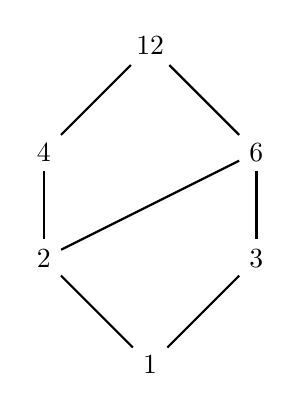
\begin{tikzpicture}[scale=0.9, thick]
            \node (1) at (0,0) {$1$};
            \node (2) at (-1.5,1.5) {$2$};
            \node (3) at (1.5,1.5) {$3$};
            \node (4) at (-1.5,3) {$4$};
            \node (6) at (1.5,3) {$6$};
            \node (12) at (0,4.5) {$12$};
            
            \draw (1) -- (2); 
            \draw (1) -- (3);
            \draw (2) -- (4); 
            \draw (2) -- (6); 
            \draw (3) -- (6);
            \draw (4) -- (12); 
            \draw (6) -- (12);
        \end{tikzpicture}
    \end{center}
\end{frame}

% Slide 16: Hasse Diagram Example 2
\begin{frame}{Hasse Diagram 2: Subset Relation}
    \textbf{Example 2: Power Set of $\{a, b\}$} \\
    \hspace*{1.5em}Let $S$ be the power set of $\{a, b\}$, and the relation $\preceq$ be the subset inclusion ($\subseteq$).
    \[ S = \{\emptyset, \{a\}, \{b\}, \{a, b\}\} \]
    
    \begin{center}
        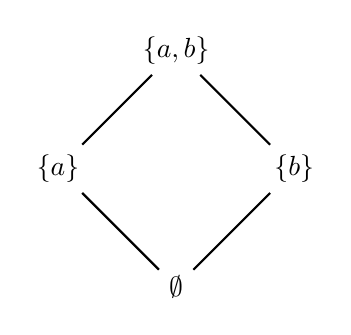
\begin{tikzpicture}[scale=1, thick]
            \node (E) at (0,0) {$\emptyset$};
            \node (A) at (-1.5,1.5) {$\{a\}$};
            \node (B) at (1.5,1.5) {$\{b\}$};
            \node (AB) at (0,3) {$\{a, b\}$};
            
            \draw (E) -- (A); 
            \draw (E) -- (B);
            \draw (A) -- (AB); 
            \draw (B) -- (AB);
        \end{tikzpicture}
    \end{center}
\end{frame}

% Slide 17: Hasse Diagram Example 3
\begin{frame}{Hasse Diagram 3: Total Order (Chain)}
    \textbf{Example 3: Less-than-or-equal-to} \\
    \hspace*{1.5em}Let $S$ be the first four natural numbers, and the relation $\preceq$ be the standard less-than-or-equal-to ($\le$). This forms a strict chain because every element is comparable.
    \[ S = \{1, 2, 3, 4\} \]
    
    \begin{center}
        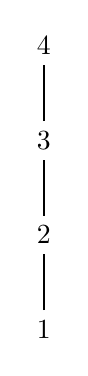
\begin{tikzpicture}[scale=1, thick]
            \node (1) at (0,0) {$1$};
            \node (2) at (0,1.2) {$2$};
            \node (3) at (0,2.4) {$3$};
            \node (4) at (0,3.6) {$4$};
            
            \draw (1) -- (2) -- (3) -- (4);
        \end{tikzpicture}
    \end{center}
\end{frame}

% Slide 18: Hasse Diagram Example 4
\begin{frame}{Hasse Diagram 4: Boolean Algebra (Cube Structure)}
    \textbf{Example 4: Divisors of 30} \\
    \hspace*{1.5em}Let $S$ be the set of positive divisors of 30, and the relation $\preceq$ be ``divides''. This creates a 3-dimensional cube structure in the Hasse Diagram.
    \[ S = \{1, 2, 3, 5, 6, 10, 15, 30\} \]
    
    \begin{center}
        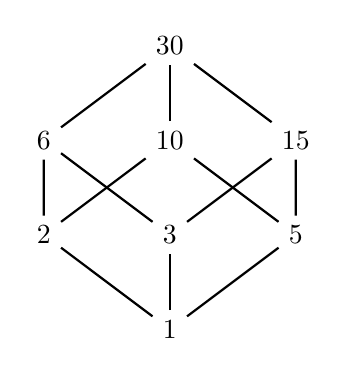
\begin{tikzpicture}[scale=0.8, thick]
            \node (1) at (0,0) {$1$};
            \node (2) at (-2,1.5) {$2$};
            \node (3) at (0,1.5) {$3$};
            \node (5) at (2,1.5) {$5$};
            \node (6) at (-2,3) {$6$};
            \node (10) at (0,3) {$10$};
            \node (15) at (2,3) {$15$};
            \node (30) at (0,4.5) {$30$};
            
            \draw (1)--(2); \draw (1)--(3); \draw (1)--(5);
            \draw (2)--(6); \draw (2)--(10);
            \draw (3)--(6); \draw (3)--(15);
            \draw (5)--(10); \draw (5)--(15);
            \draw (6)--(30); \draw (10)--(30); \draw (15)--(30);
        \end{tikzpicture}
    \end{center}
\end{frame}

% Slide 19: Hasse Diagram Example 5
\begin{frame}{Hasse Diagram 5: Antichain}
    \textbf{Example 5: Equality Relation} \\
    \hspace*{1.5em}Let $S$ be a set of discrete elements, and the relation $\preceq$ be strict equality ($=$). Because no two distinct elements are comparable, no edges are drawn.
    \[ S = \{a, b, c, d\} \]
    
    \vspace{0.8cm}
    
    \begin{center}
        \begin{tikzpicture}[scale=1, thick]
            \node (a) at (-3,0) {$a$};
            \node (b) at (-1,0) {$b$};
            \node (c) at (1,0) {$c$};
            \node (d) at (3,0) {$d$};
            % No lines are drawn because elements are only related to themselves
        \end{tikzpicture}
    \end{center}
\end{frame}

% Slide 20: Thank You
\begin{frame}
    \centering
    \Huge \textbf{Thank You!}
\end{frame}

\end{document}
